\documentclass{beamer}
\usepackage[utf8]{inputenc}

\def\dt{\partial t}
\def\dx{\partial x}
\def\dy{\partial y}

\def\dz{\partial z}
\def\BE{\begin{equation}}
\def\EE{\end{equation}}
\def\half{\frac{1}{2}}
\def\calT{\cal T}
\def\Deltax{\Delta x}
\def\Deltat{\Delta t}
\DeclareSymbolFont{largesymbolsA}{U}{txexa}{m}{n}
\DeclareMathSymbol{\varprod}{\mathop}{largesymbolsA}{16}
\setbeamerfont{caption}{size=\scriptsize}

\title{Analyzing Complex Models using Data and Statistics}

\author{A.K. Patra, \inst{1} \and A. Bevilacqua, \inst{2} \and A. Akhavan Safaei \inst{3}}
\institute[University at Buffalo]{\inst{1} Dept. of Mech. and  Aero. Eng. \and \inst{2} Dept. of Earth Sciences \and \inst{3}Comp. Data Science and Eng.}

\date[ICCS 2018]{International Conference on Computational Sciences, 2018}

\begin{document}

\frame{\titlepage}



\begin{frame}
\frametitle{Models and assumptions}
\textbf{What is a Model?}
\begin{quote}{\it A model is a representation of a postulated relationship among inputs and outputs of a system, usually informed by observation and based on a hypothesis that best explains the relationship.}\end{quote}
\vskip.5cm
\begin{itemize}
\item models depend on a {\it hypothesis}, and,
\item models use the {\it data from observation} to validate and refine the hypothesis.
\end{itemize}
\end{frame}
  
  
\begin{frame}
\frametitle{Analysis Process - \small{in \emph{predictive mode}}}
We are interested in the general predictive capabilities of the models, related to the outcomes over a whole range.
\vskip.3cm
\begin{itemize}
  \item Stage 1: Parameter Ranges $P_M\left(p_1,\dots,p_{N_M}\right)\sim \bigotimes_{i=1}^{N_M} Unif(a_{i,M},b_{i,M}).$
  \vskip.5cm
  \item Stage 2: Simulations and Data Gathering
\end{itemize}
\vskip-.5cm
\begin{figure}[H]
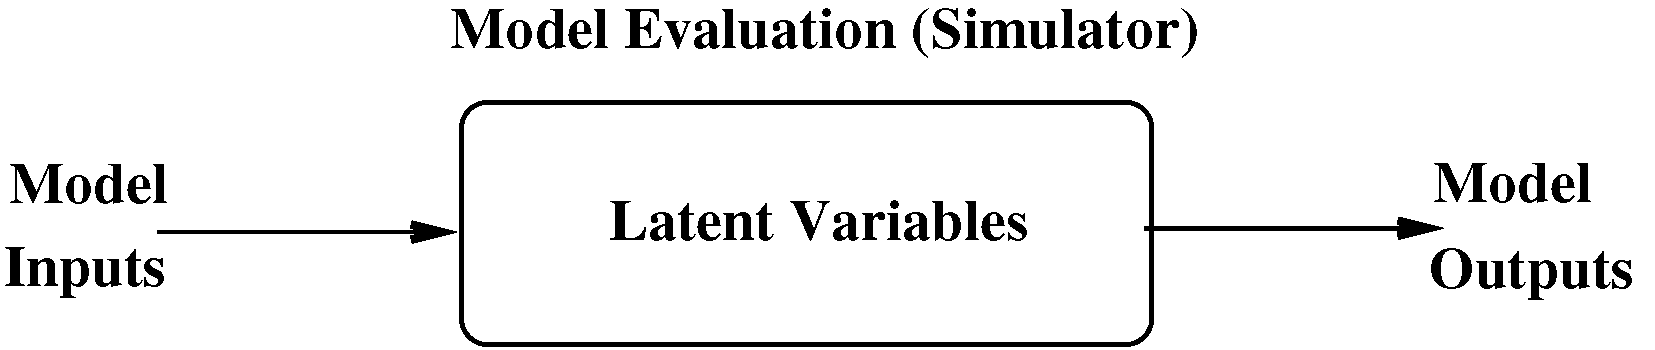
\includegraphics[width=0.85\textwidth]{figures/modelproc.png}
\caption{Models and variables}
\end{figure}
\begin{itemize}
  \item Stage 3: Results Analysis
\end{itemize}
\end{frame}


\begin{frame}
\frametitle{Statistics of latent variables - \small{dominance factors}}
Dominance factors provide insight into the dominance of a particular latent variable over the others.
\vskip.5cm
\begin{definition}[dominance factors]
Let $(F_i)_{i\in I}$ be random variables on $(\Omega, \mathcal F, P_M)$. Then, $\forall i$, the dominant variable is defined as:
$$\Phi:=\left\{
    \begin{array}{ll}
      \max_i |F_i|, & \hbox{if not null;} \\
      1, & \hbox{otherwise.}
    \end{array}
  \right.$$
In particular, for each $j \in I$, the dominance factors are defined as:
$$p_j:=P_M\left\{\Phi=|F_j|\right\}.$$
\end{definition}
\end{frame}

\begin{frame}
\frametitle{Statistics of latent variables - \small{expected contributions}}
Random contributions are obtained dividing the latent variables by $\Phi$, and hence belong to $[0,1]$.
\vskip.5cm
\begin{definition}[expected contributions]
Let $(F_i)_{i\in I}$ be random variables on $(\Omega, \mathcal F, P_M)$. Then, $\forall i$, the random contribution is defined as:
$$C_i:=\frac{F_i}{\Phi},$$
where $\Phi$ is the dominant variable. Thus, $\forall i$, the expected contributions are defined by $E\left[C_i\right]$.
\end{definition}
\end{frame}


\begin{frame}
\frametitle{Modeling of geophysical mass flows}
The depth-averaged Saint-Venant equations that result are:
\small{
\begin{eqnarray}
\label{eq:D_A}
\frac{\partial h}{\partial t} +
\frac{\partial}{\partial x}(h \bar{u}) +
\frac{\partial}{\partial y}(h\bar{v}) &=& 0 \nonumber \\
\frac{\partial}{\partial t} (h\bar{u}) +
\frac{\partial}{\partial x}\left(h\bar{u}^2 + \frac{1}{2}k g_{z}h^2\right) + \frac{\partial}{\partial y}(h\bar{u}\bar{v}) &=& S_{x}\\
\frac{\partial}{\partial t} (h\bar{v}) +
\frac{\partial}{\partial x}(h\bar{u}\bar{v}) +
\frac{\partial}{\partial y}\left(h\bar{v}^2 + \frac{1}{2}k g_{z}h^2\right) &=& S_{y} \nonumber
\end{eqnarray}}

Source terms $S_x$, $S_y$ characterize \emph{Mohr-Coulomb} (MC), \emph{Pouliquen-Forterre} (PF) and \emph{Voellmy-Salm} (VS) models.
\end{frame}


\begin{frame}
\frametitle{Main assumptions - \small{all the models include \textit{curvature effects}}.}
\textbf{Mohr-Coulomb}
\begin{itemize}
\item \textit{Basal Friction} based on a constant friction angle.
\item \textit{Internal Friction} based on a constant friction angle.
\end{itemize}

\textbf{Pouliquen-Forterre}
\begin{itemize}
\item \textit{Basal Friction} is based on an interpolation of two different friction angles, based on the flow regime and depth.
\item Normal stress is modified by a \textit{hydrostatic pressure force} related to the flow height gradient.
\end{itemize}

\textbf{Voellmy-Salm}
\begin{itemize}
\item \textit{Basal Friction} is based on a constant coefficient, similarly to the MC rheology.
\item Additional \textit{turbulent friction} is based on the local velocity by a quadratic expression.
\end{itemize}
\end{frame}


\begin{frame}
\frametitle{Overview of the case studies}
\begin{figure}
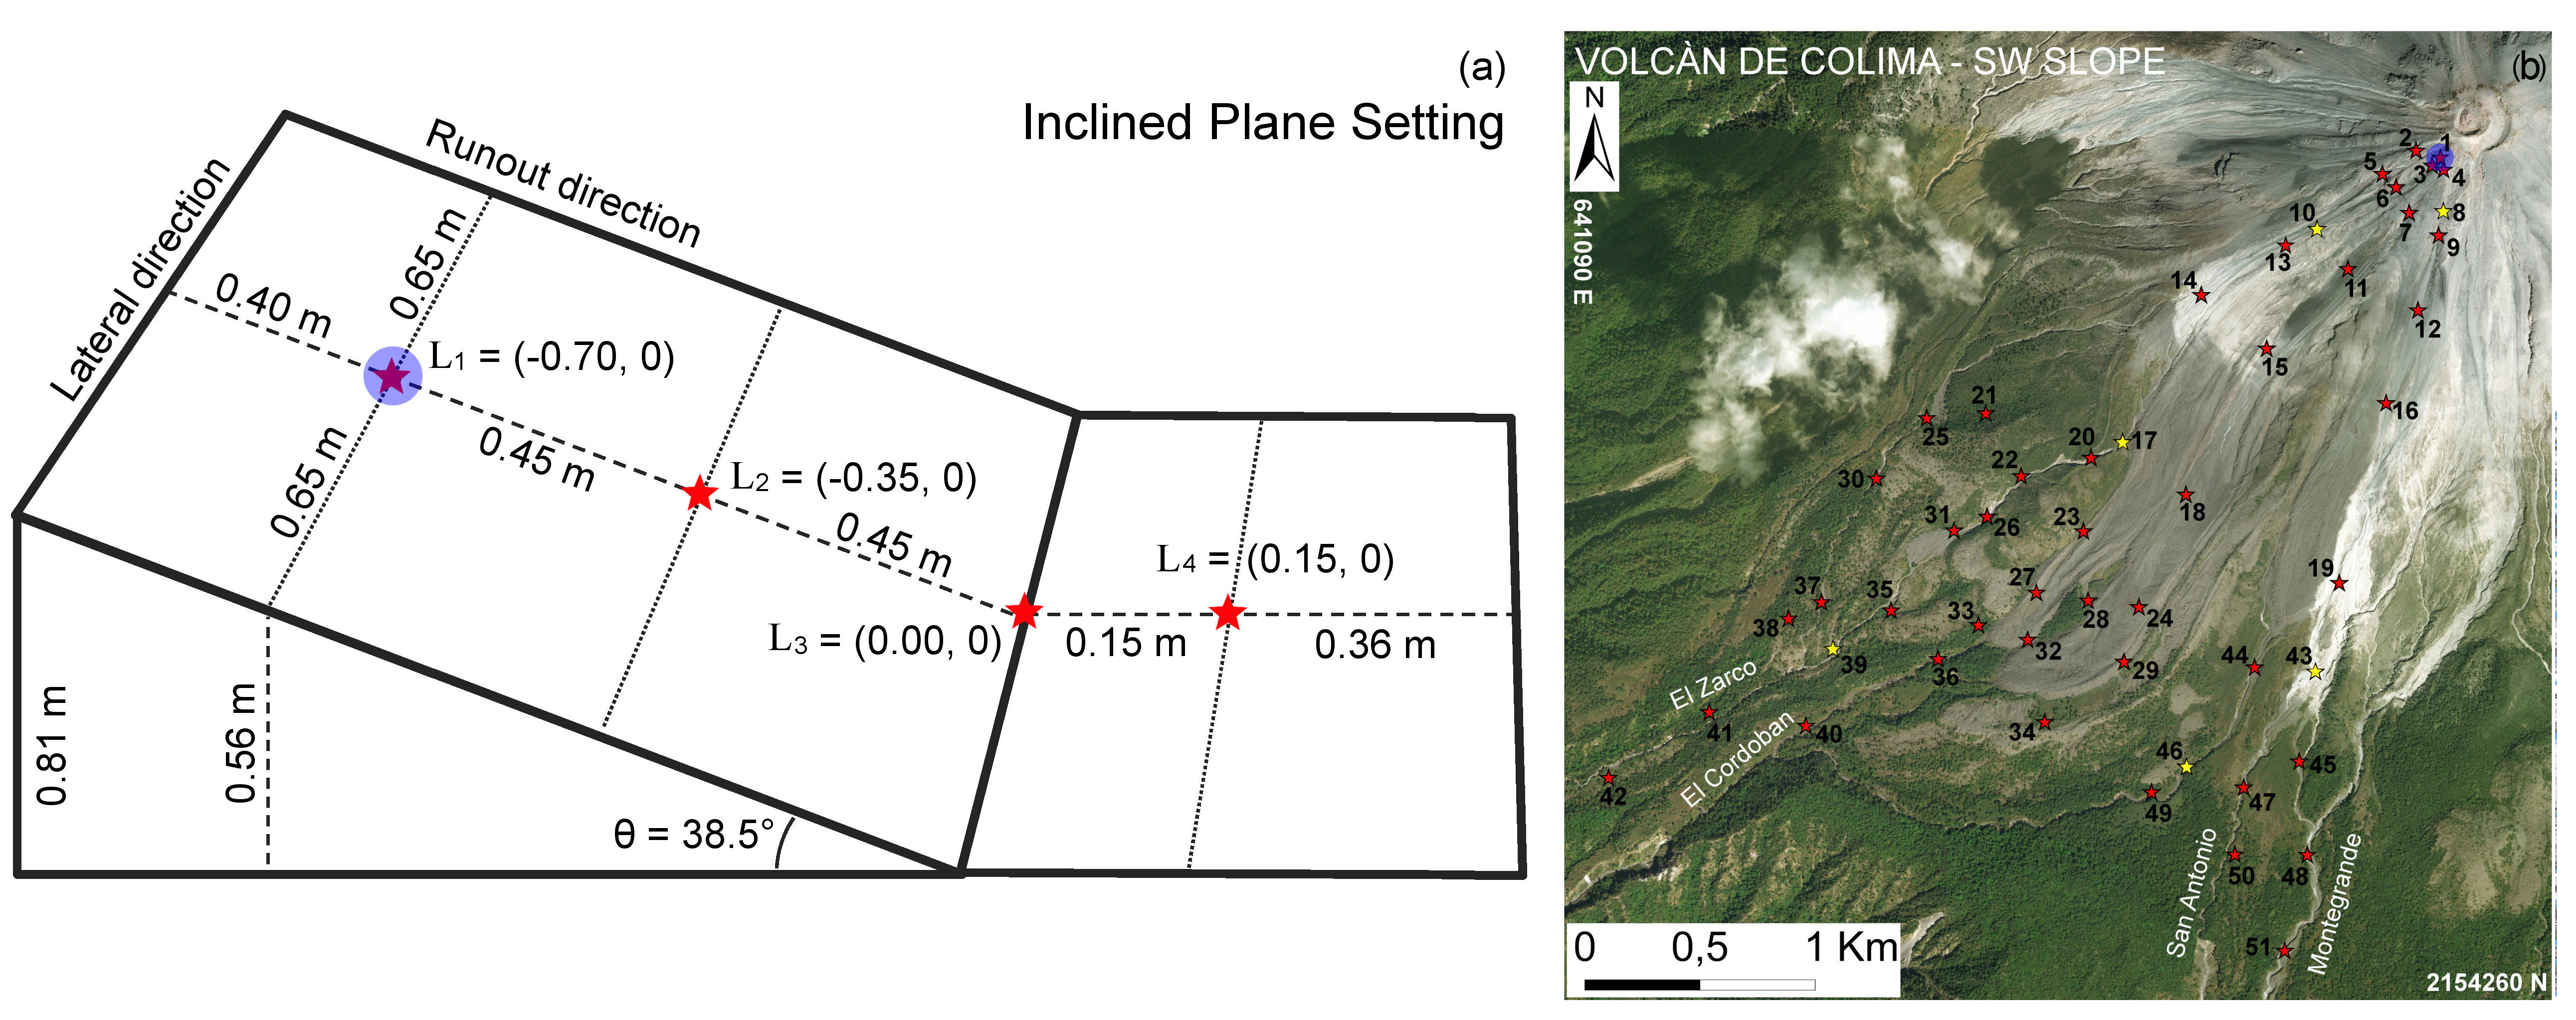
\includegraphics[width=0.95\textwidth]{ChineseFig.jpeg}
    \caption{{\bf [Left]} Inclined plane description, including local samples sites (red stars). Pile location is marked by a blue dot.{\bf [Right]}(a) Volc{\'a}n de Colima (M{\'e}xico) overview, including 51 numbered local sample sites (stars) and four labeled major ravines channeling the flow. Pile location is marked by a blue dot. Reported coordinates are in UTM zone 13N. Background is a satellite photo. }
\end{figure}
\end{frame}


\begin{frame}
\frametitle{Small scale flow - \small{observable outputs}}
\begin{figure}
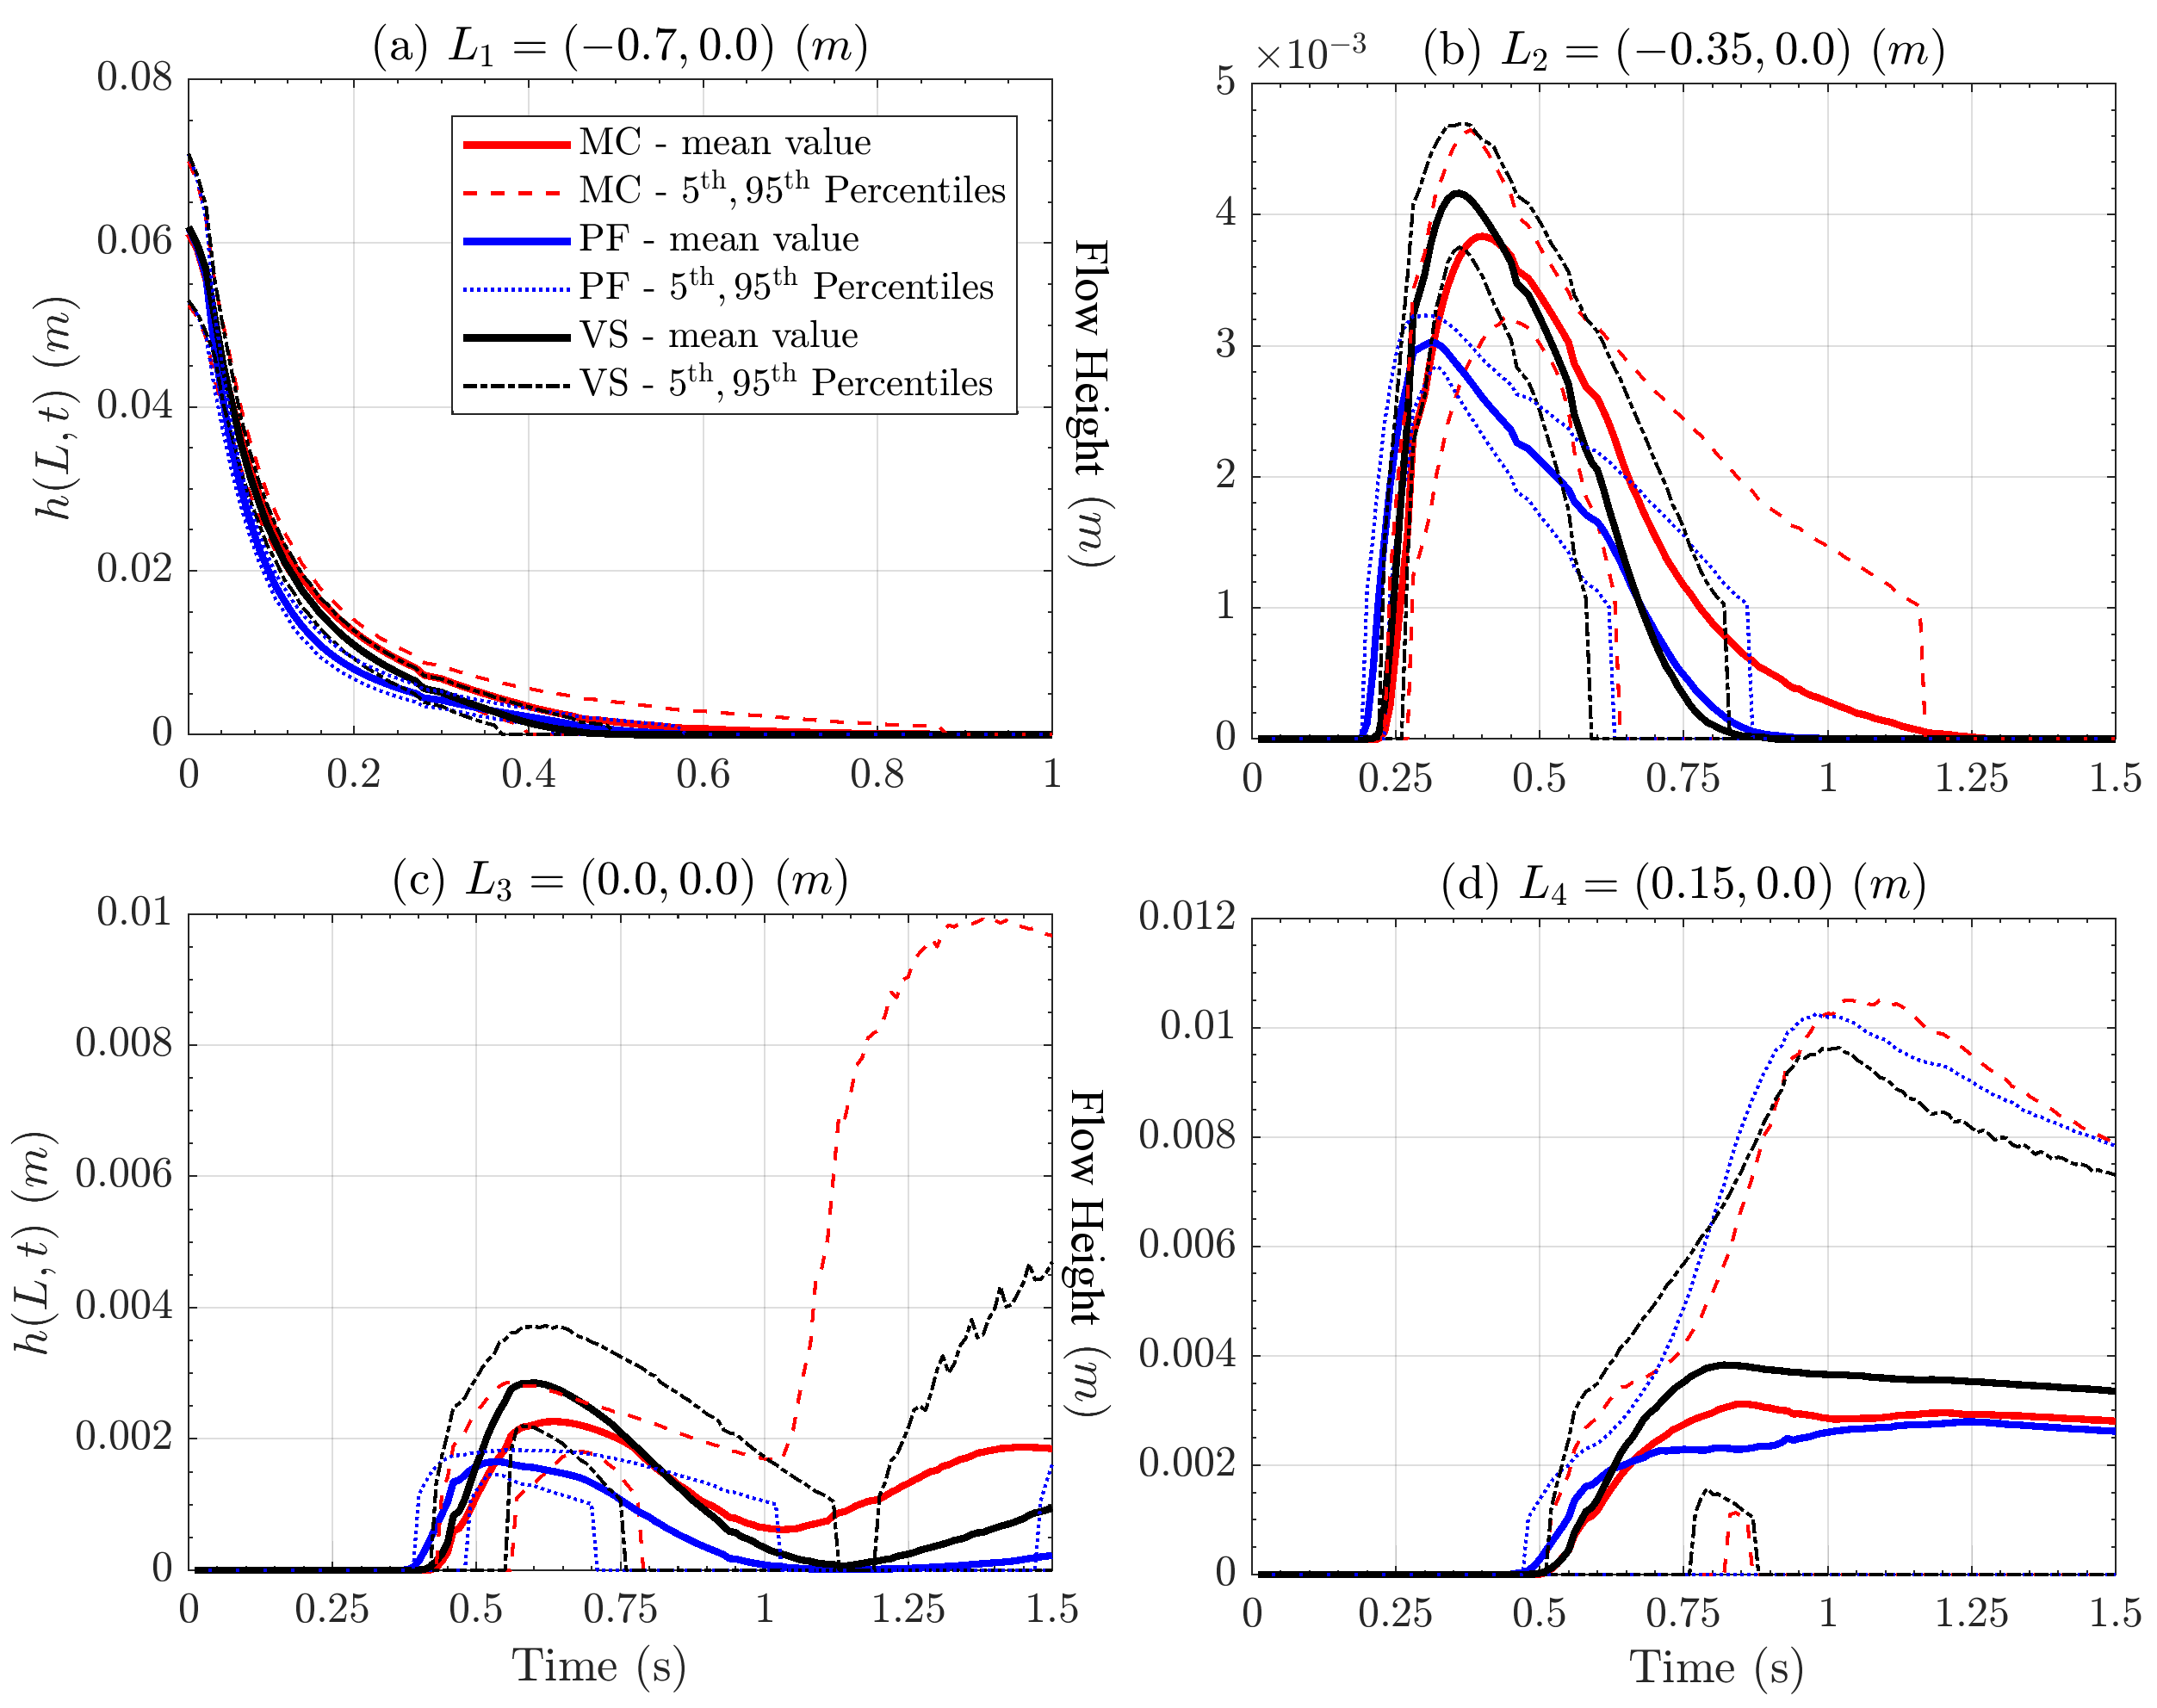
\includegraphics[width=0.75\textwidth]{figures/incline/Height.png}
        \caption{Flow height in four locations. Bold line is mean value, dashed/dotted lines are 5$^{\mathrm{th}}$ and 95$^{\mathrm{th}}$ percentile bounds. Different models are displayed with different colors. Plots are at different scale, for simplifying exposition.}
\end{figure}
\end{frame}

\begin{frame}
\frametitle{Small scale flow - \small{power integrals}}
\begin{figure}
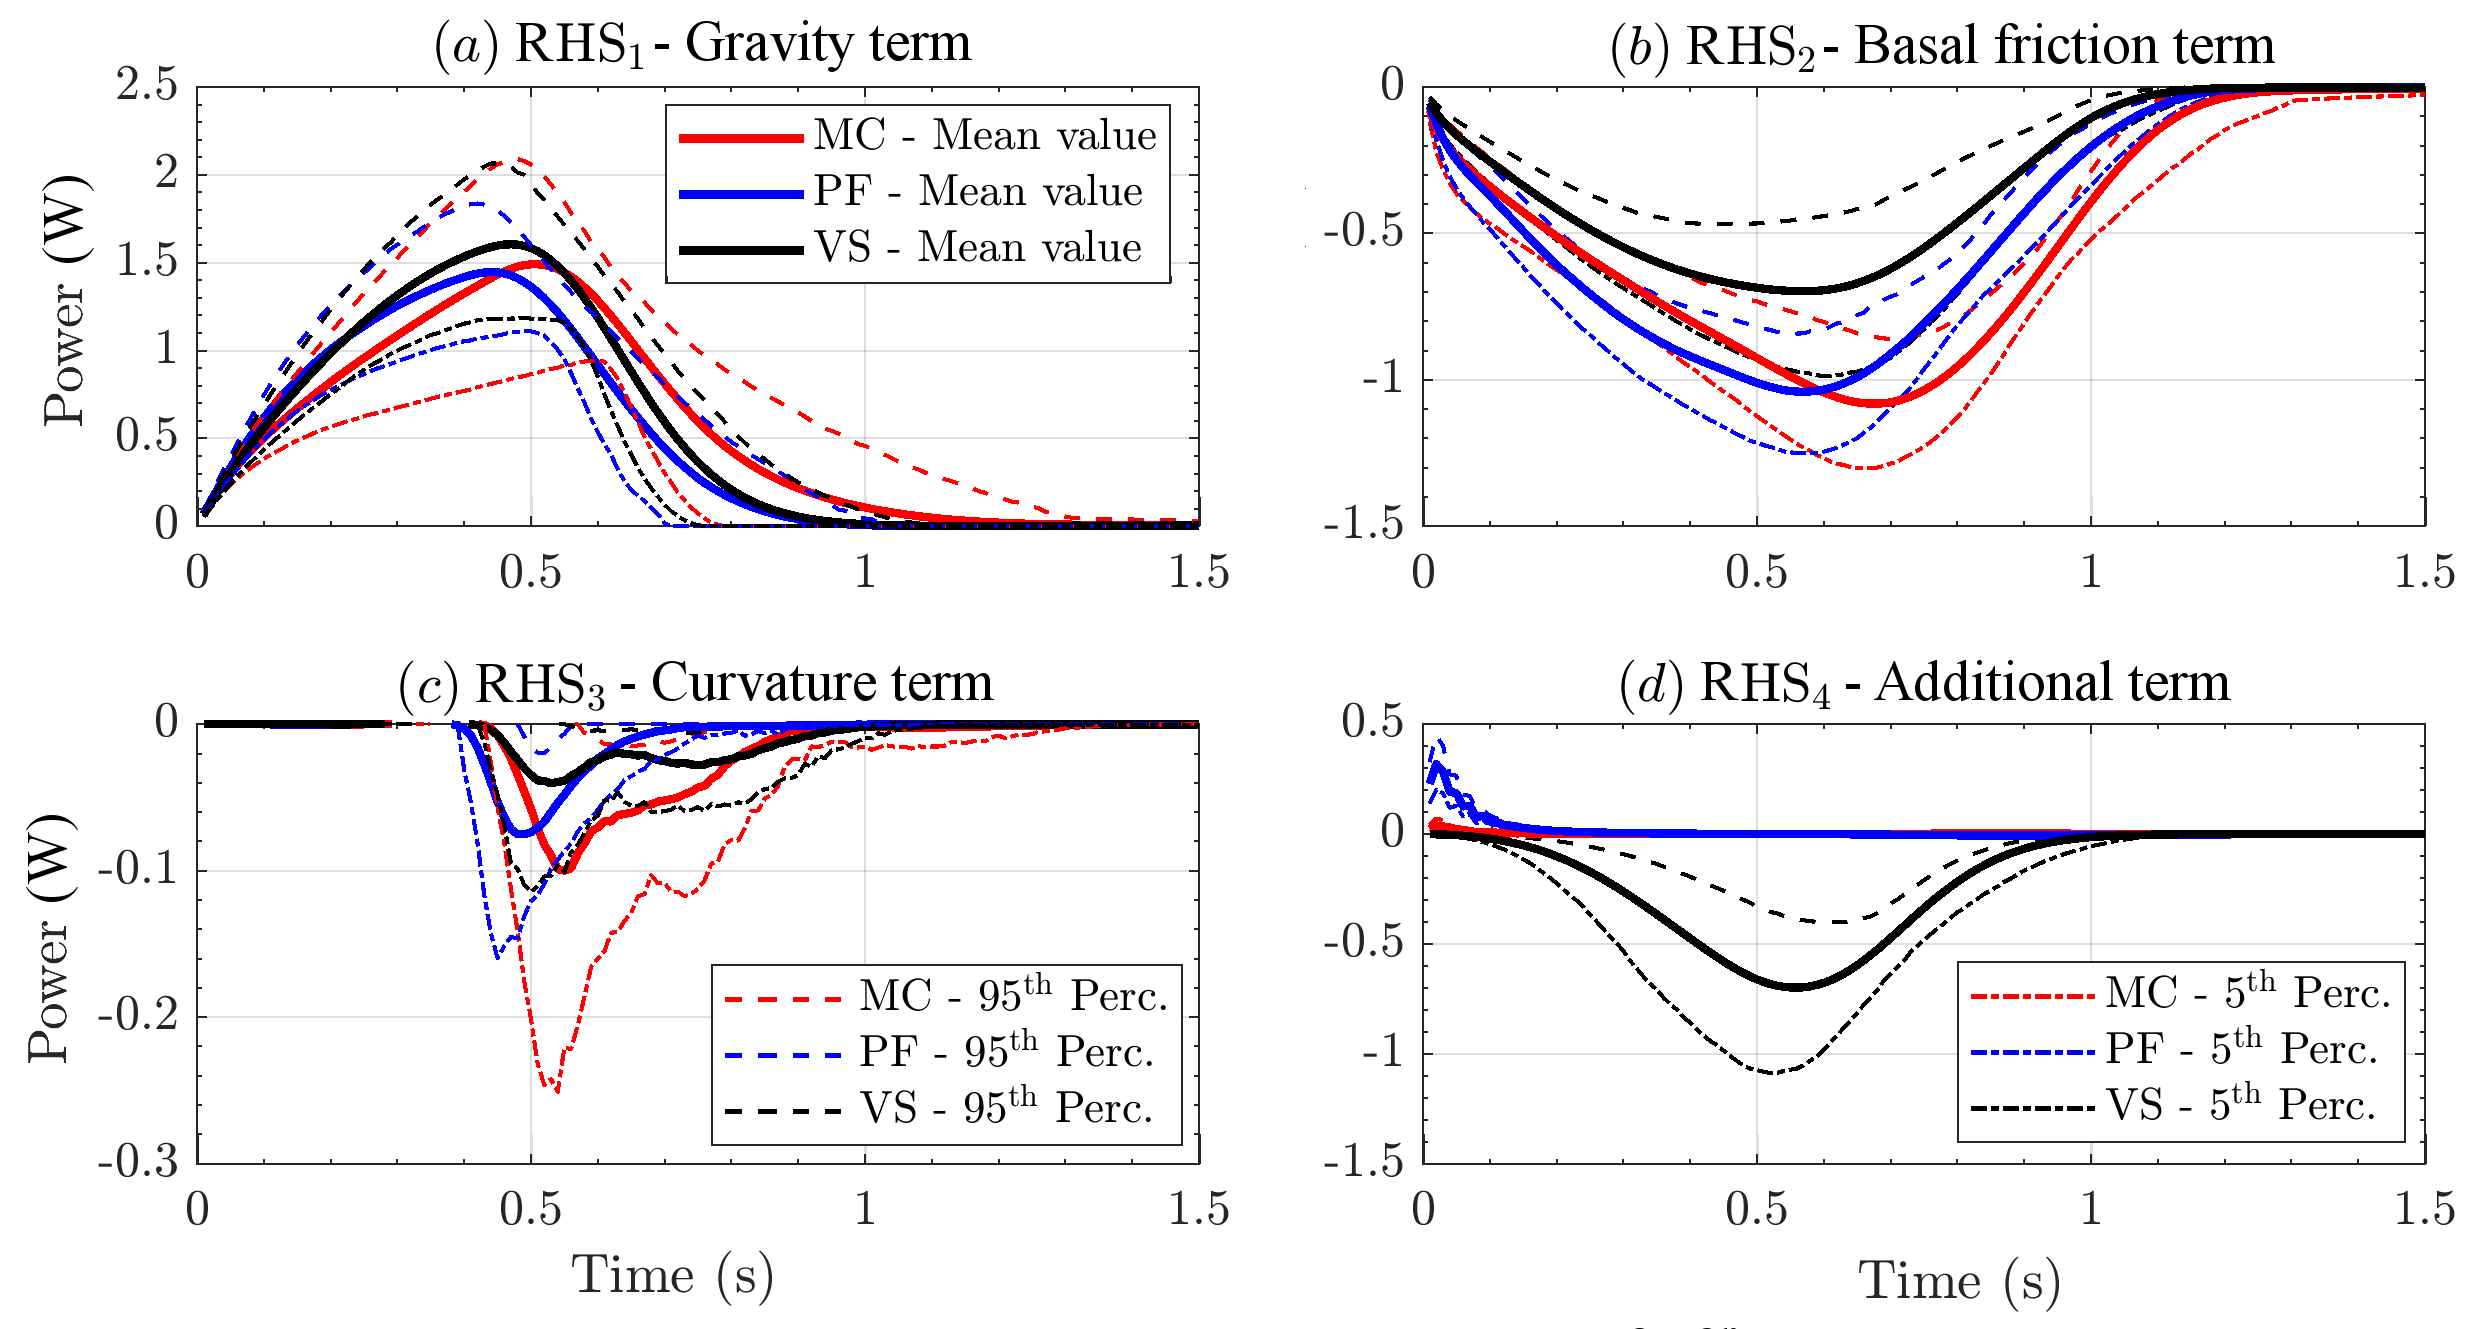
\includegraphics[width=0.95\textwidth]{figures/incline/PowersIncline.png}
        \caption{Spatial integral of the RHS powers. Bold line is mean value, dashed lines are 5$^{\mathrm{th}}$ and 95$^{\mathrm{th}}$ percentile bounds. Different models are displayed with different colors.}
\end{figure}
\end{frame}


\begin{frame}
\frametitle{Large scale flow - \small{proximal to the initial pile}}
\begin{figure}
        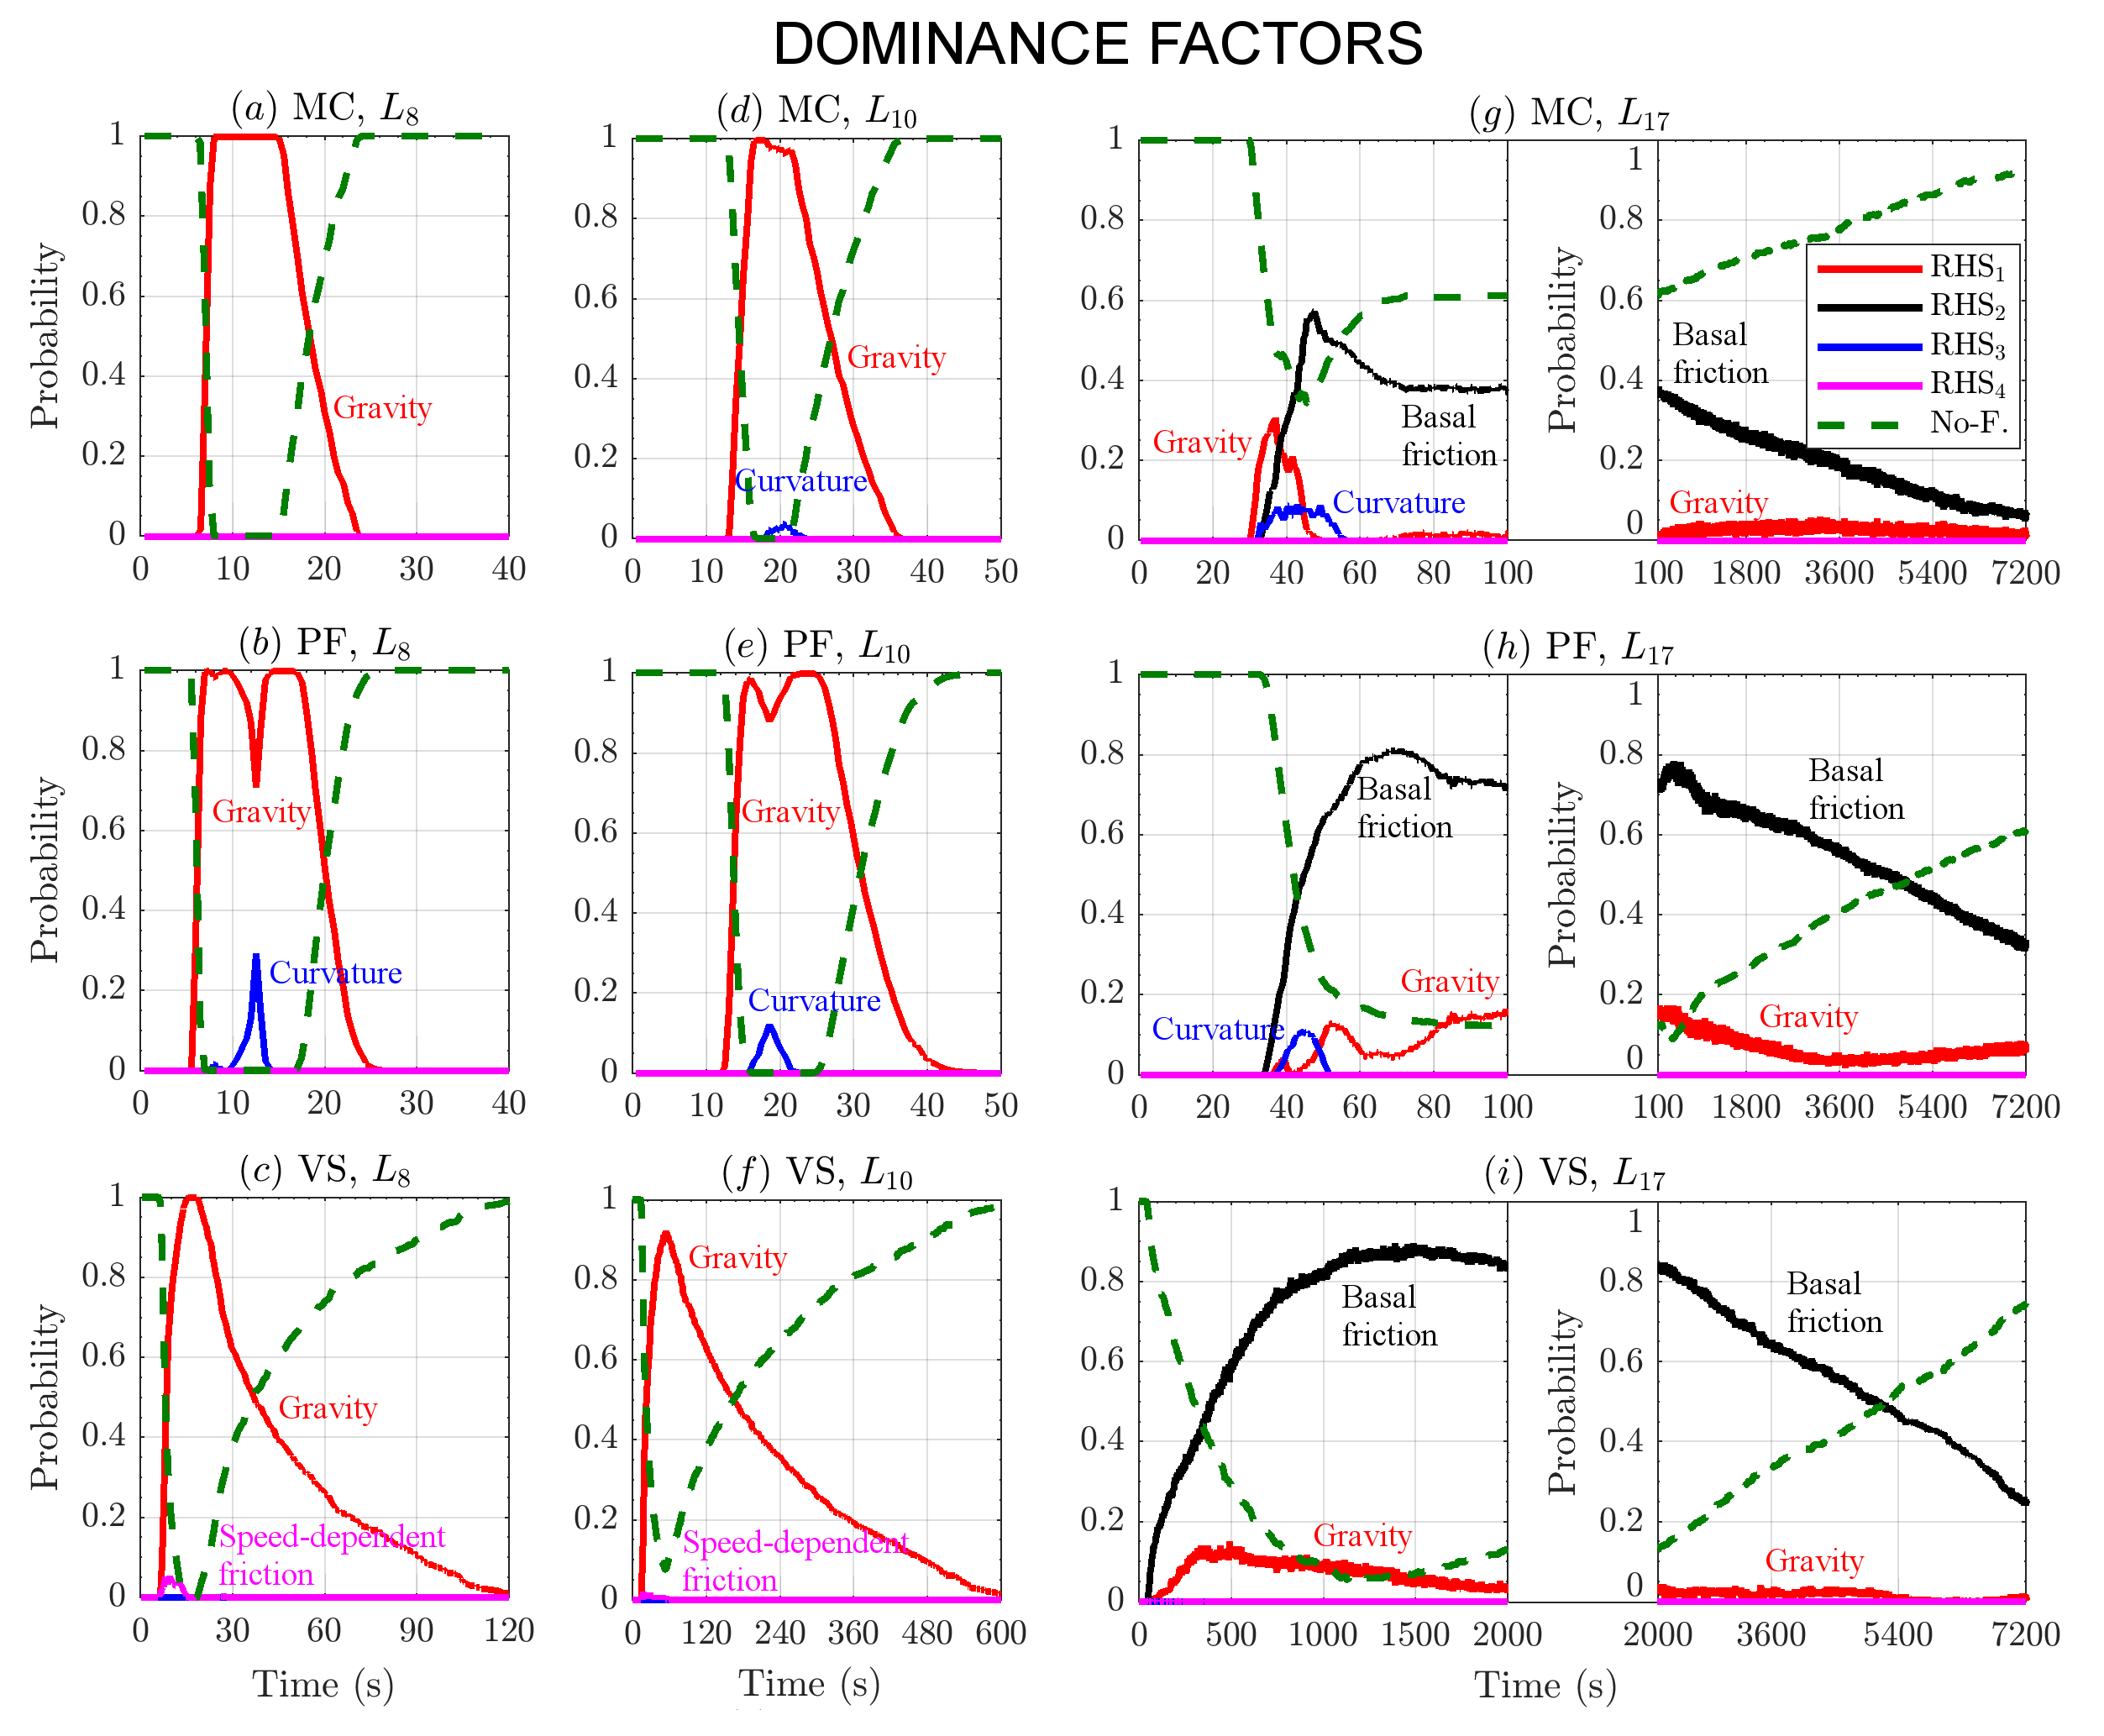
\includegraphics[width=0.75\textwidth]{figures/Colima/Pr1_total.png}
        \caption{Dominance factors of \textbf{RHS} forces in three locations in the first km of runout. Different models are plotted separately: (a,d,g) assume MC; (b,e,h) assume PF; (c,f,i) assume VS. Different colors correspond to different force terms. No-flow probability is displayed with a green dashed line.}
\end{figure}
\end{frame}

\begin{frame}
\frametitle{Large scale flow - \small{proximal to the initial pile}}
\begin{figure}
        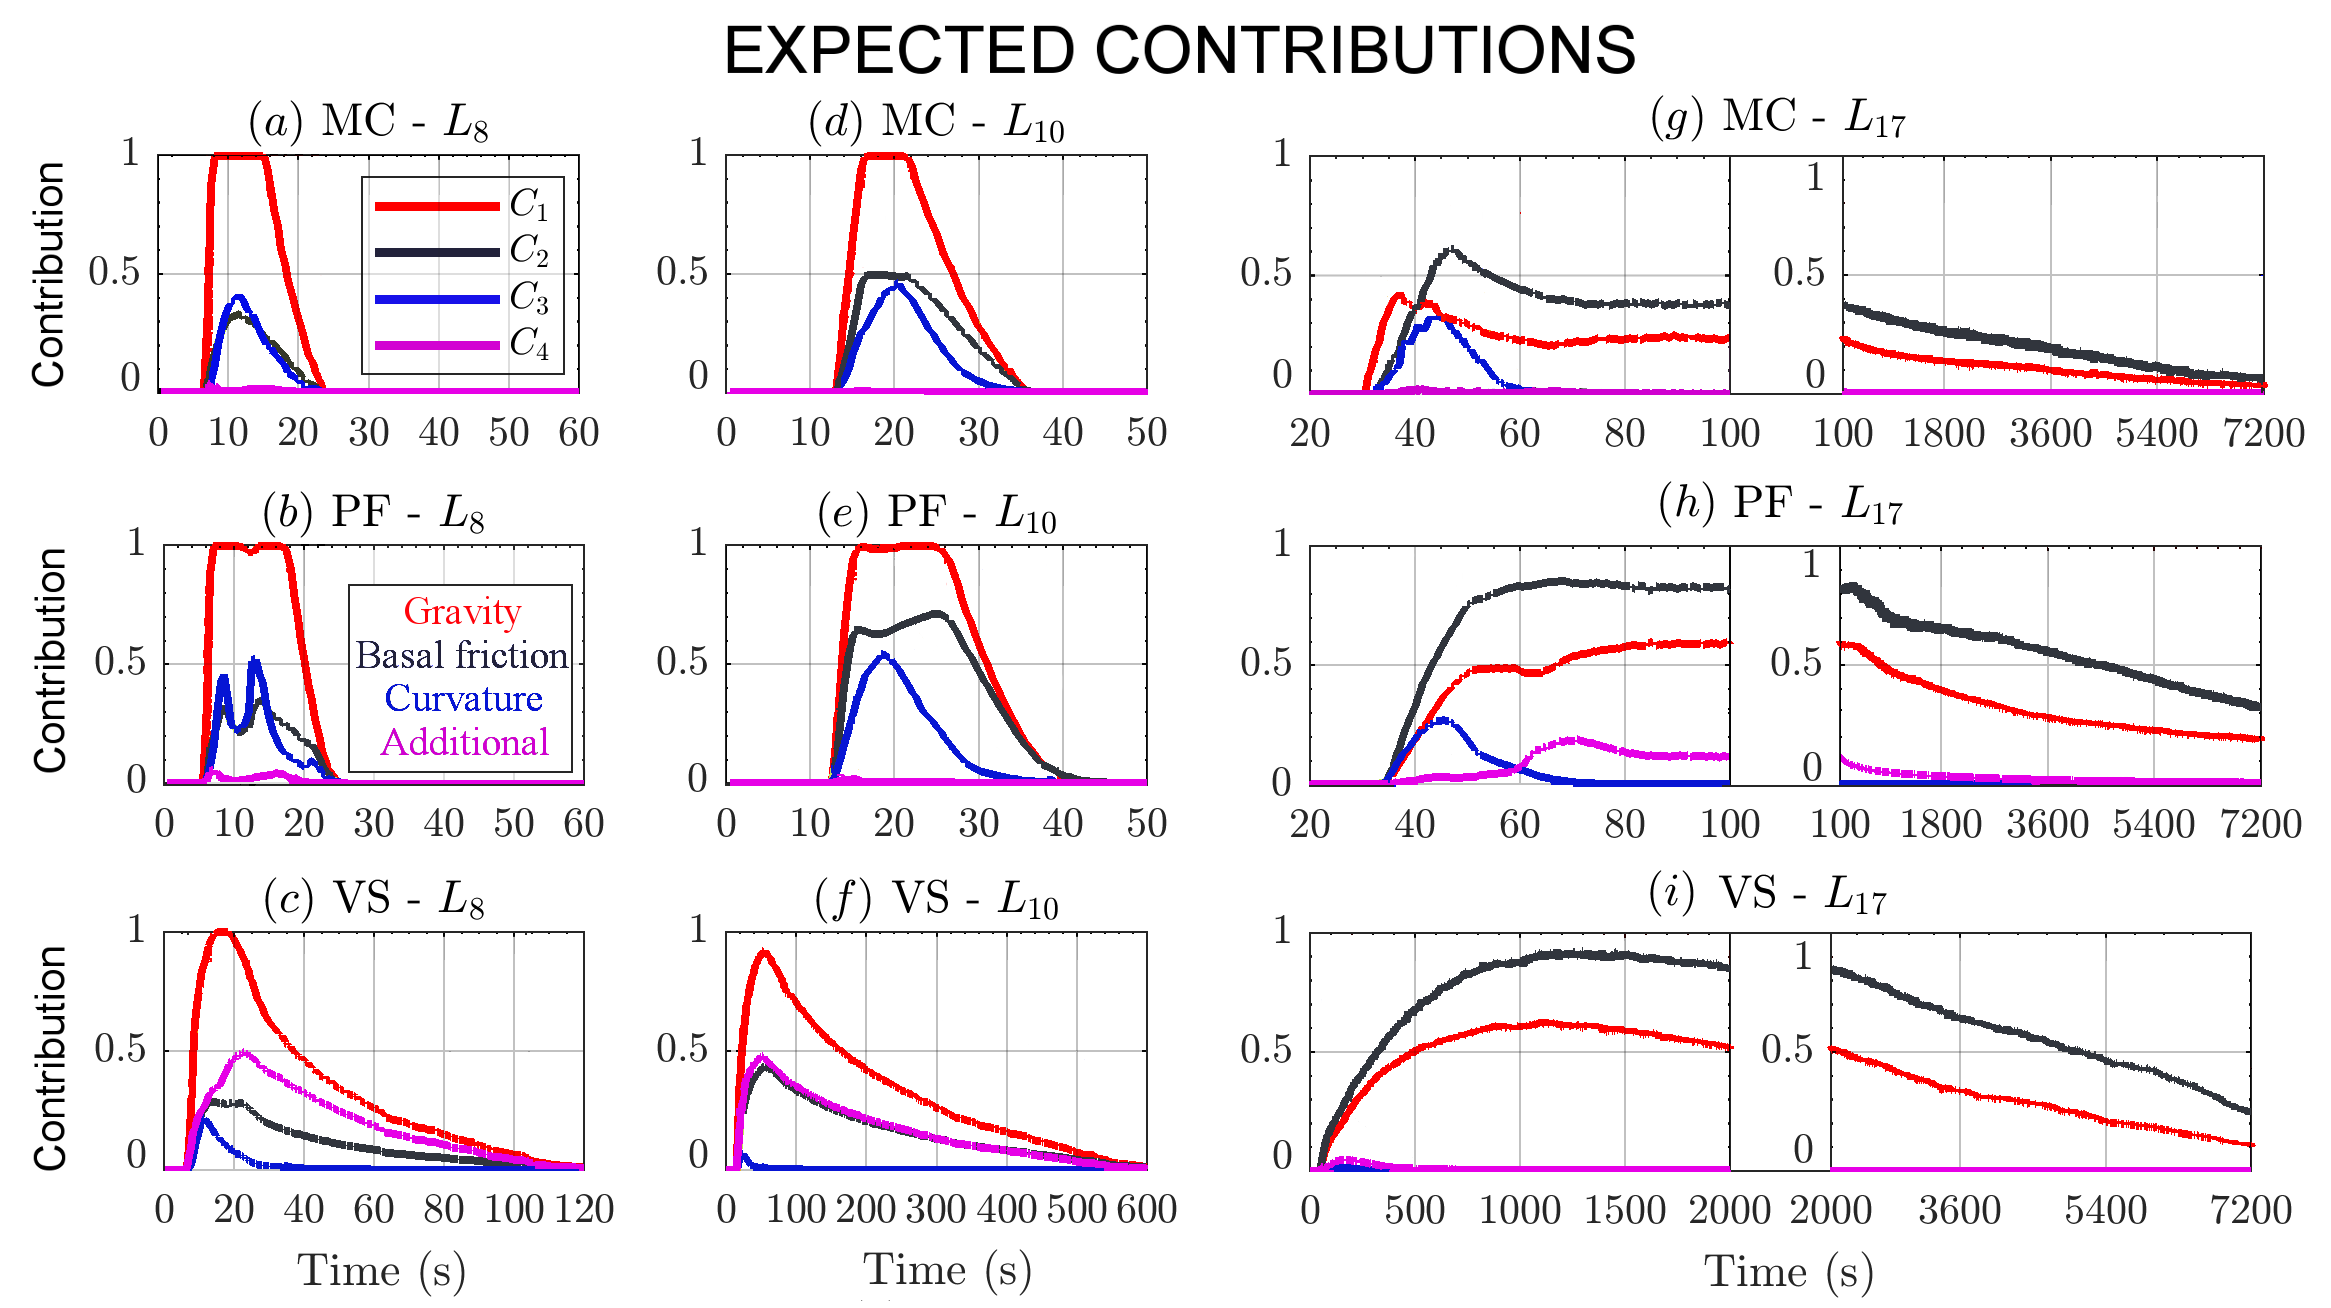
\includegraphics[width=0.85\textwidth]{figures/Colima/Ci1_total.png}
        \small{\caption{Expected contributions of \textbf{RHS} forces in three locations in the first km of runout. Different models are plotted separately: (a,d,g) assume MC; (b,e,h) assume PF; (c,f,i) assume VS. Different colors correspond to different force terms.}}
\end{figure}
\end{frame}

\begin{frame}
\frametitle{Large scale flow - \small{distal from the initial pile}}
\begin{figure}
        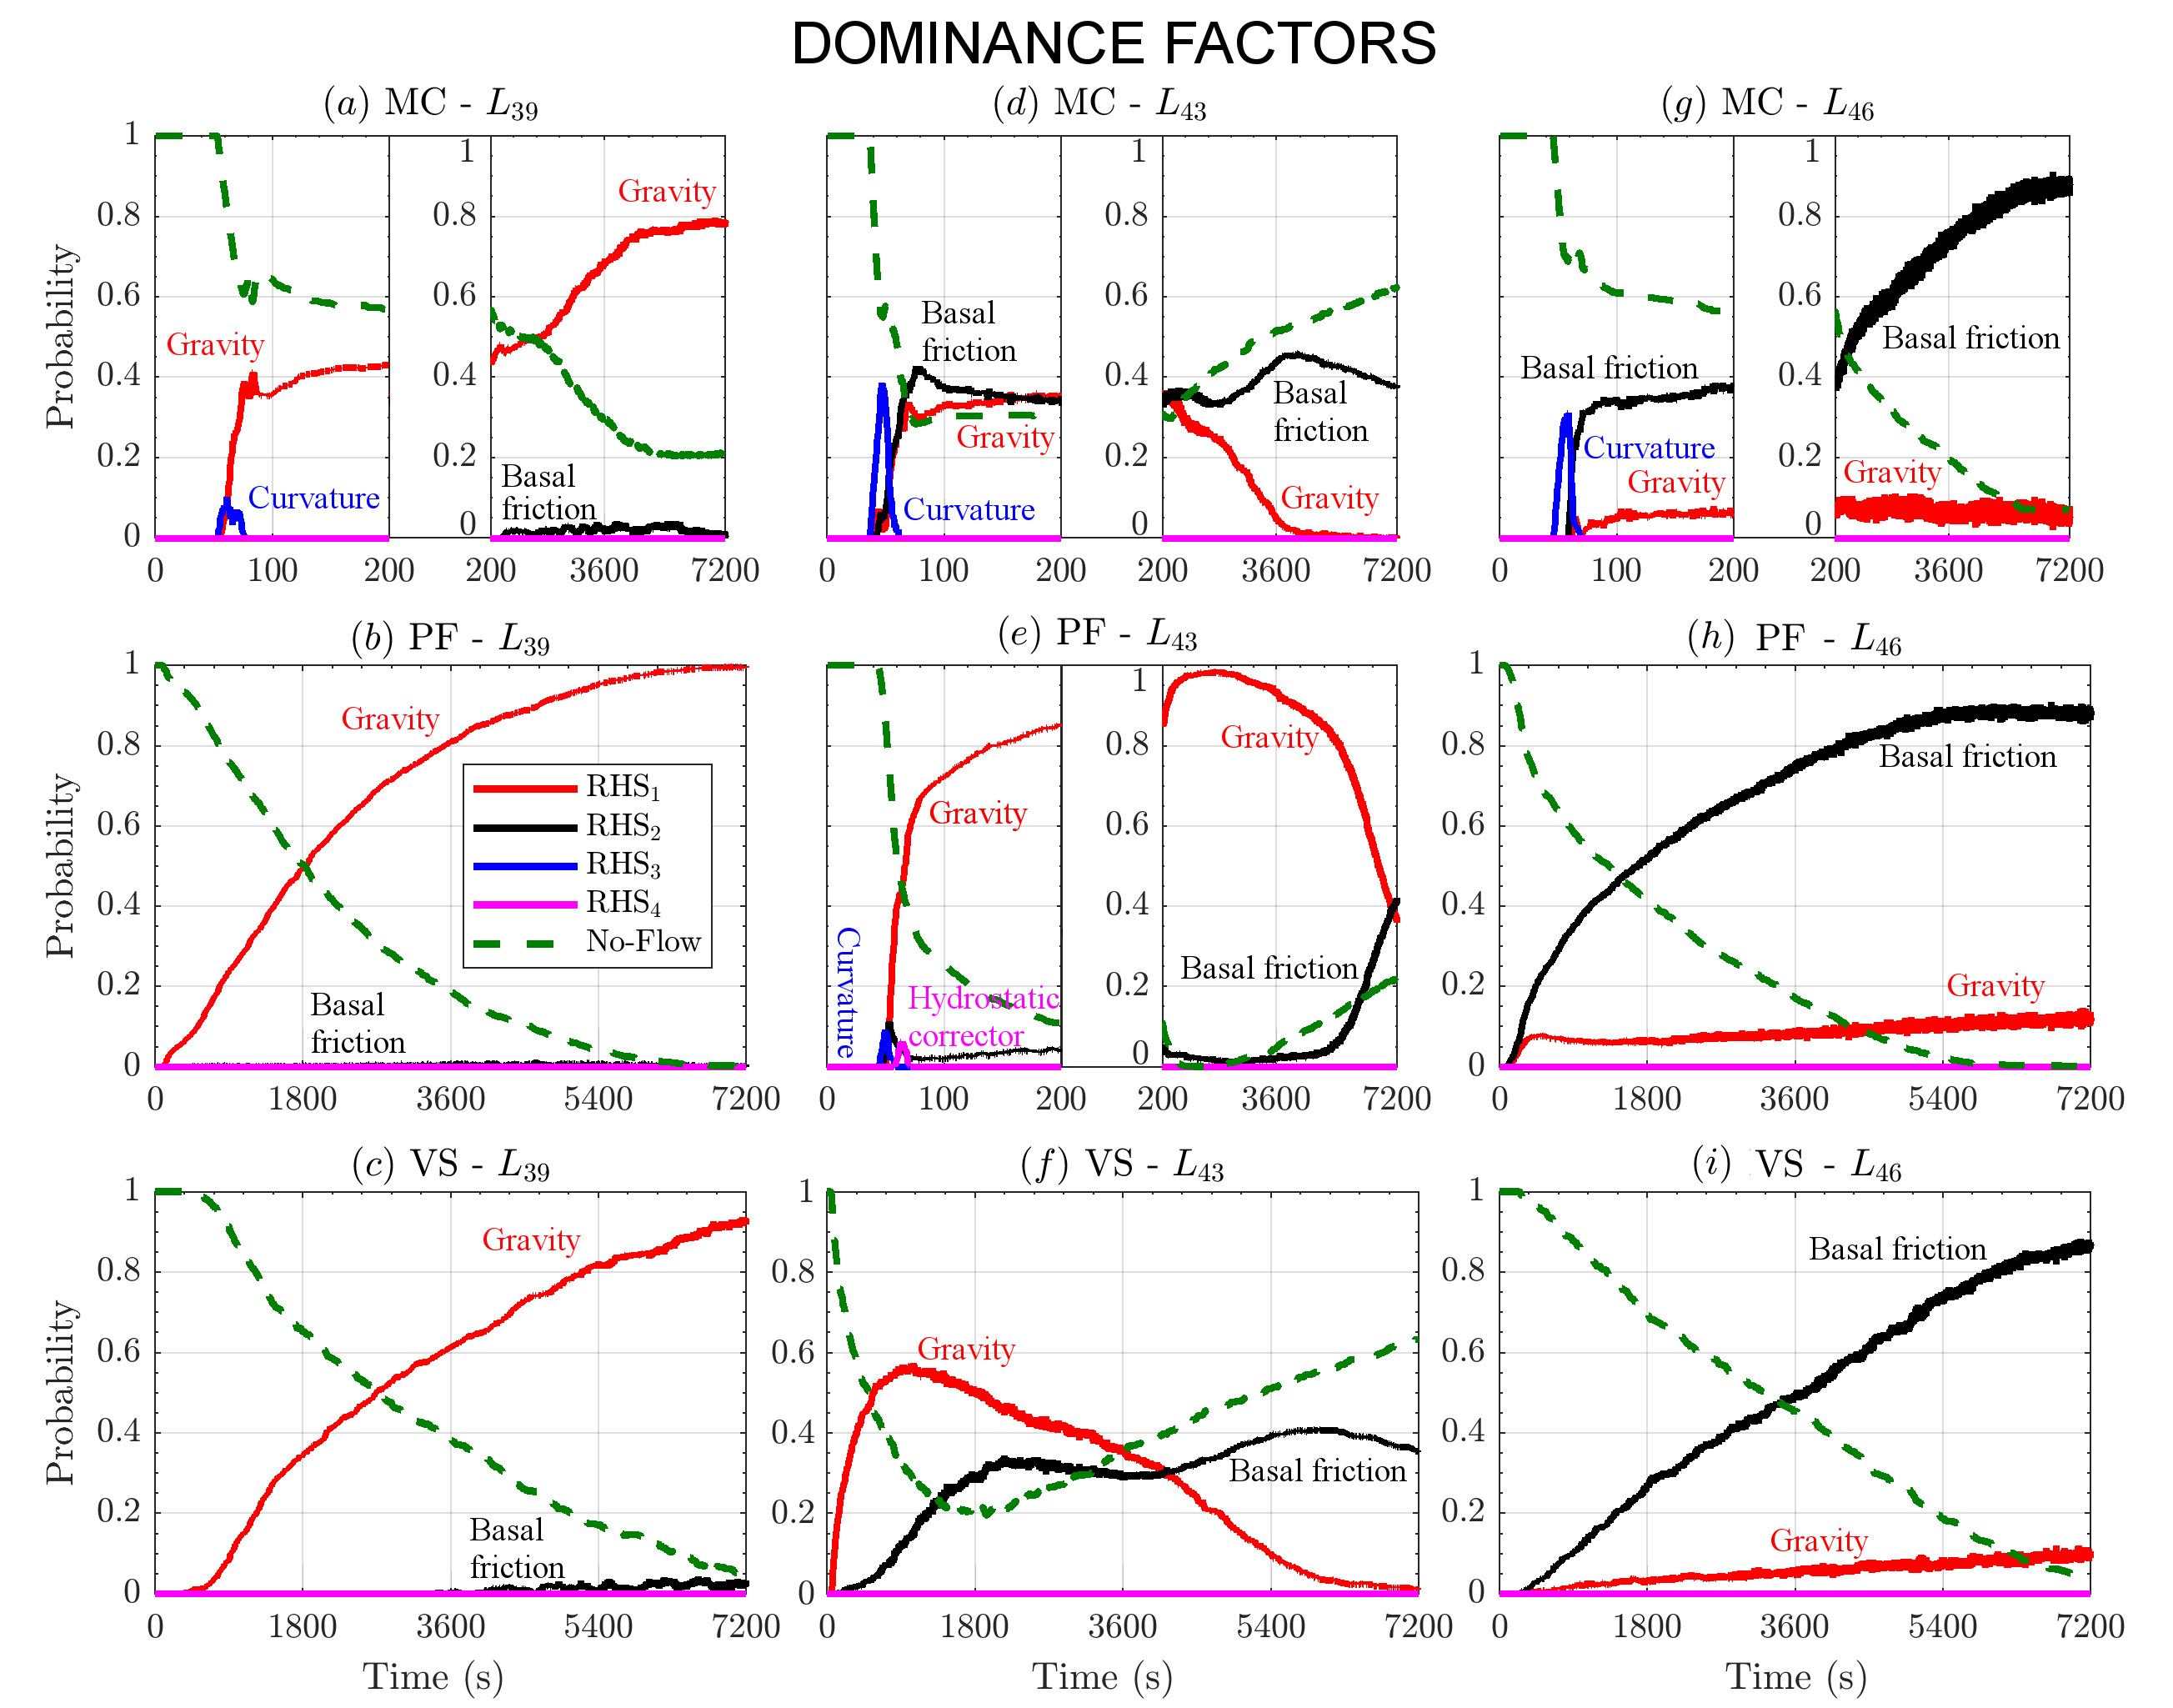
\includegraphics[width=0.75\textwidth]{figures/Colima/Pr2_total.png}
        \caption{Dominance factors of \textbf{RHS} forces in three locations after 2 km of runout. Different models are plotted separately: (a,d,g) assume MC; (b,e,h) assume PF; (c,f,i) assume VS. Different colors correspond to different force terms. No-flow probability is displayed with a green dashed line.}
\end{figure}
\end{frame}

\begin{frame}
\frametitle{Large scale flow - \small{distal from the initial pile}}
\begin{figure}
        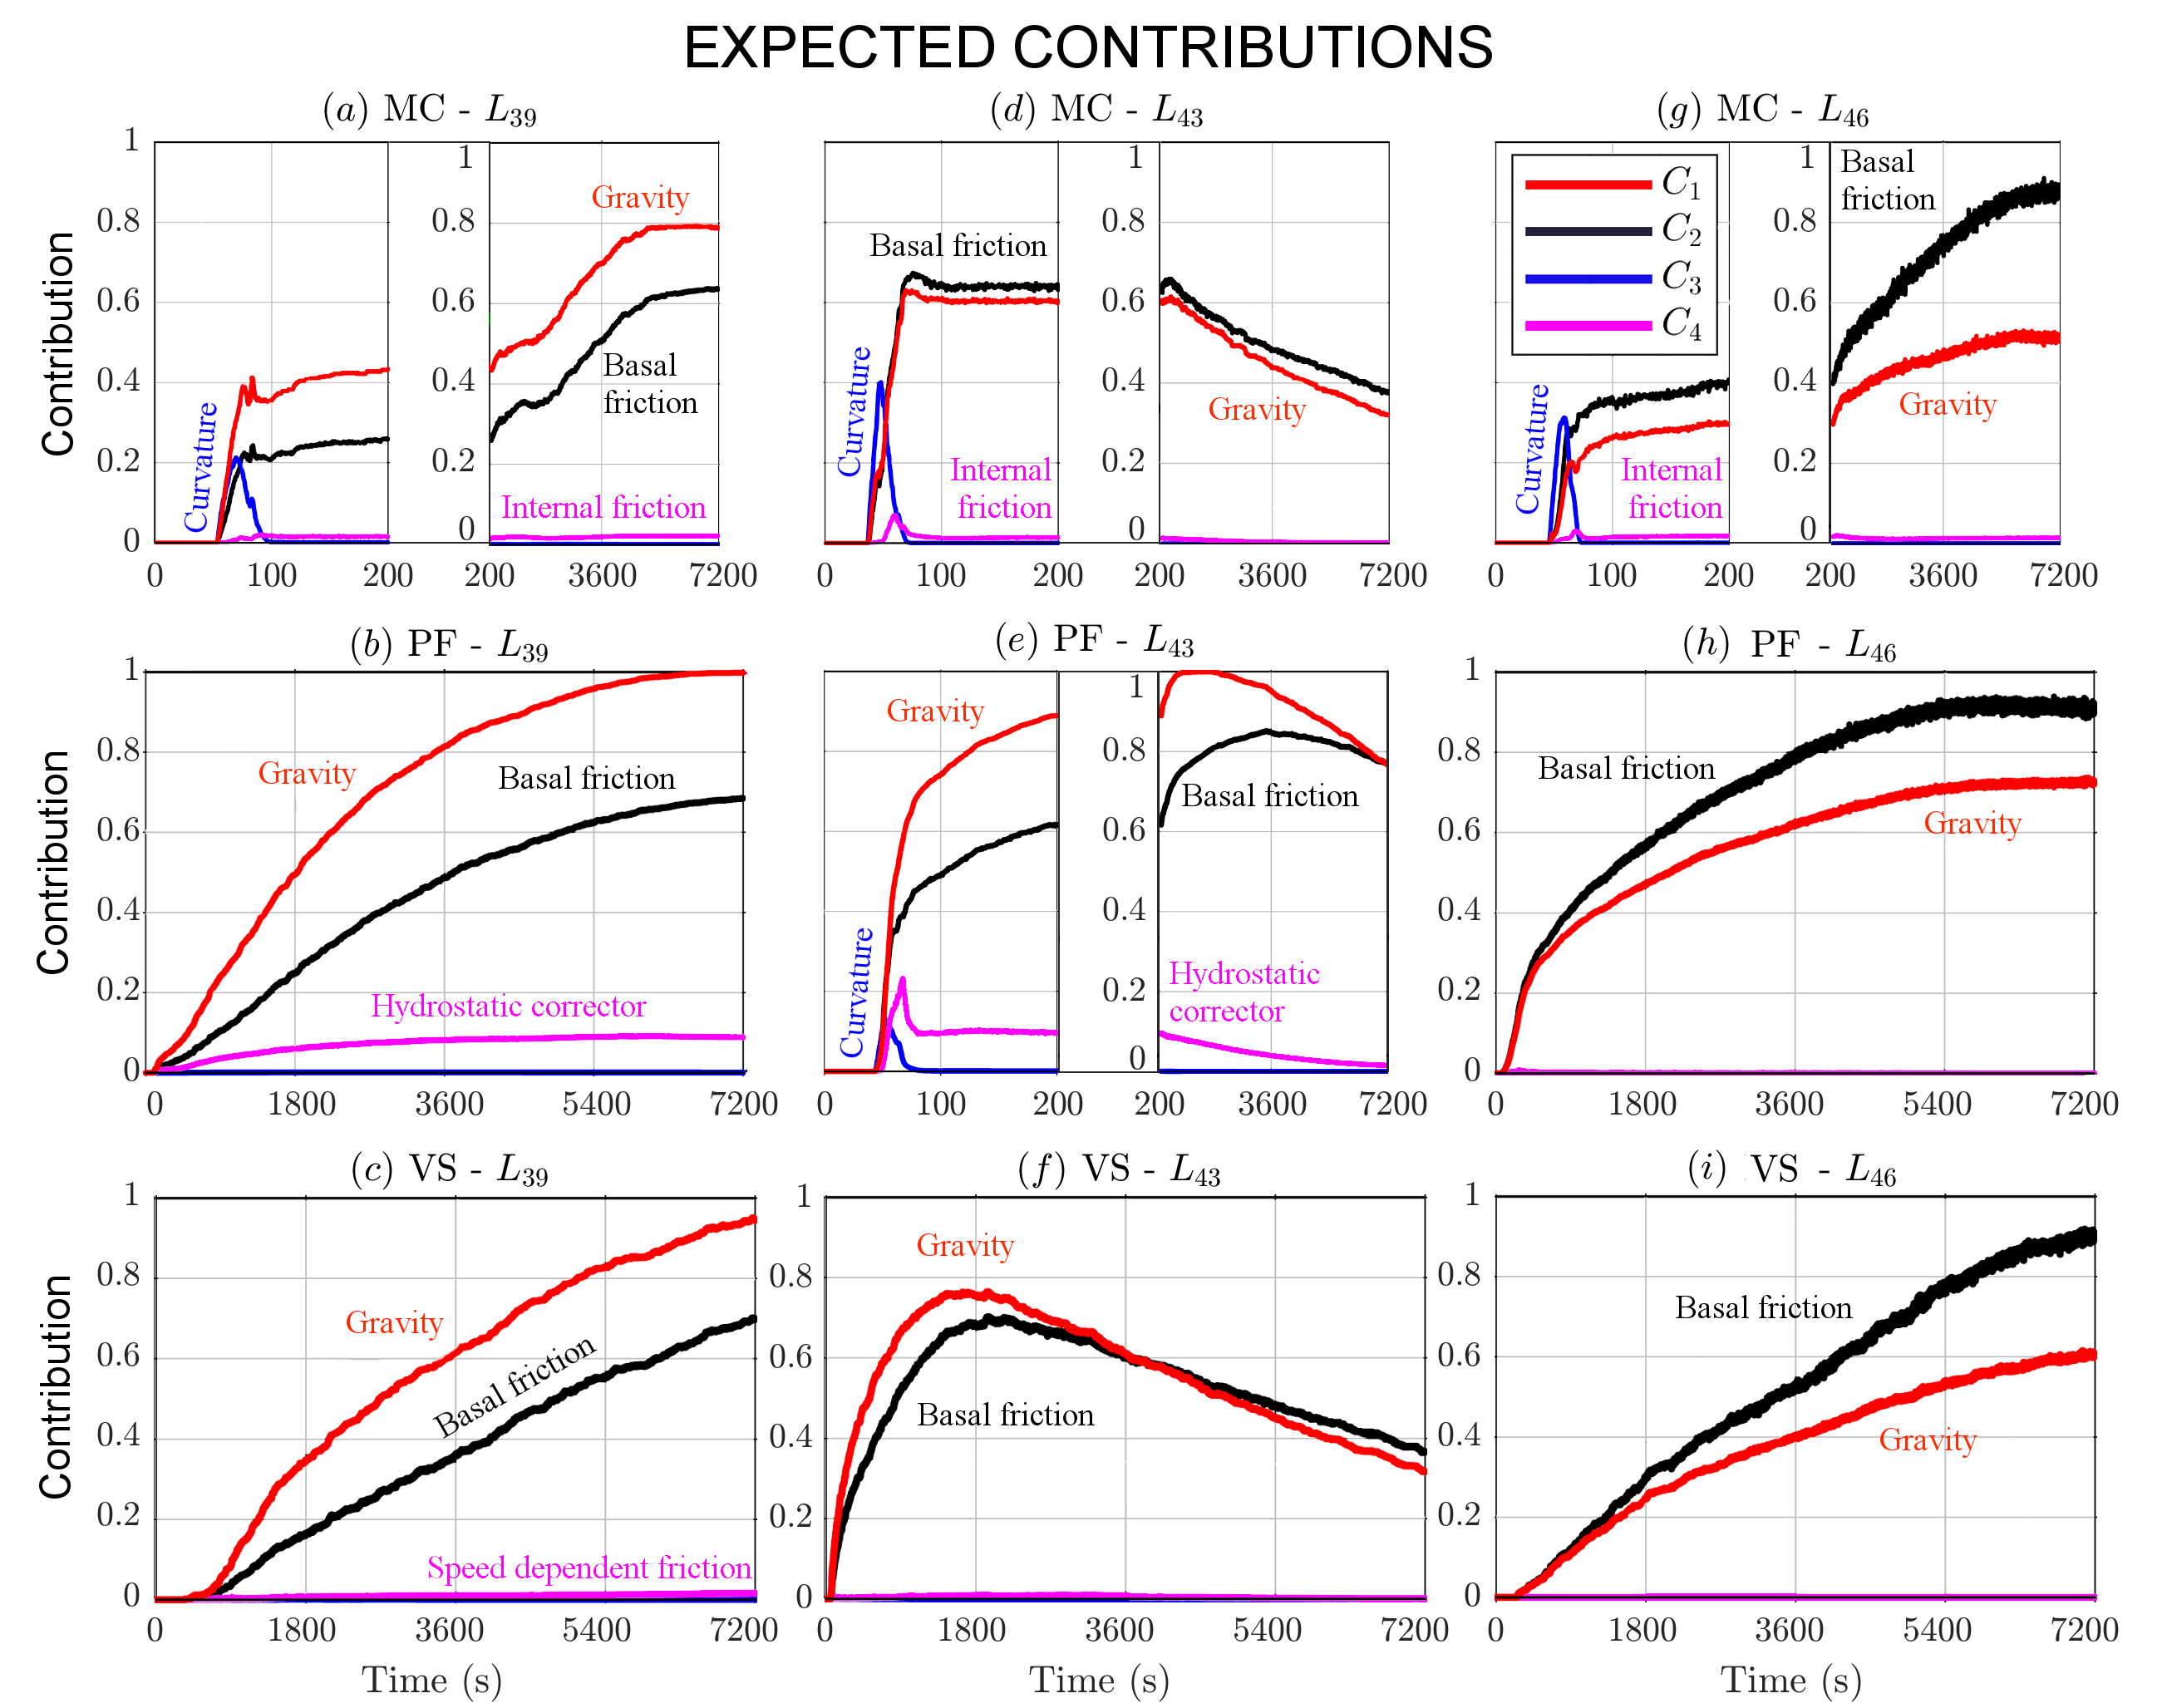
\includegraphics[width=0.75\textwidth]{figures/Colima/Ci2_total.png}
        \caption{Expected contributions of \textbf{RHS} forces in three locations after 2 km of runout. Different models are plotted separately: (a,d,g) assume MC; (b,e,h) assume PF; (c,f,i) assume VS. Different colors correspond to different force terms.}
\end{figure}
\end{frame}

\begin{frame}
\frametitle{Large scale flow - \small{flow extent and spatial integrals}}
\begin{figure}
        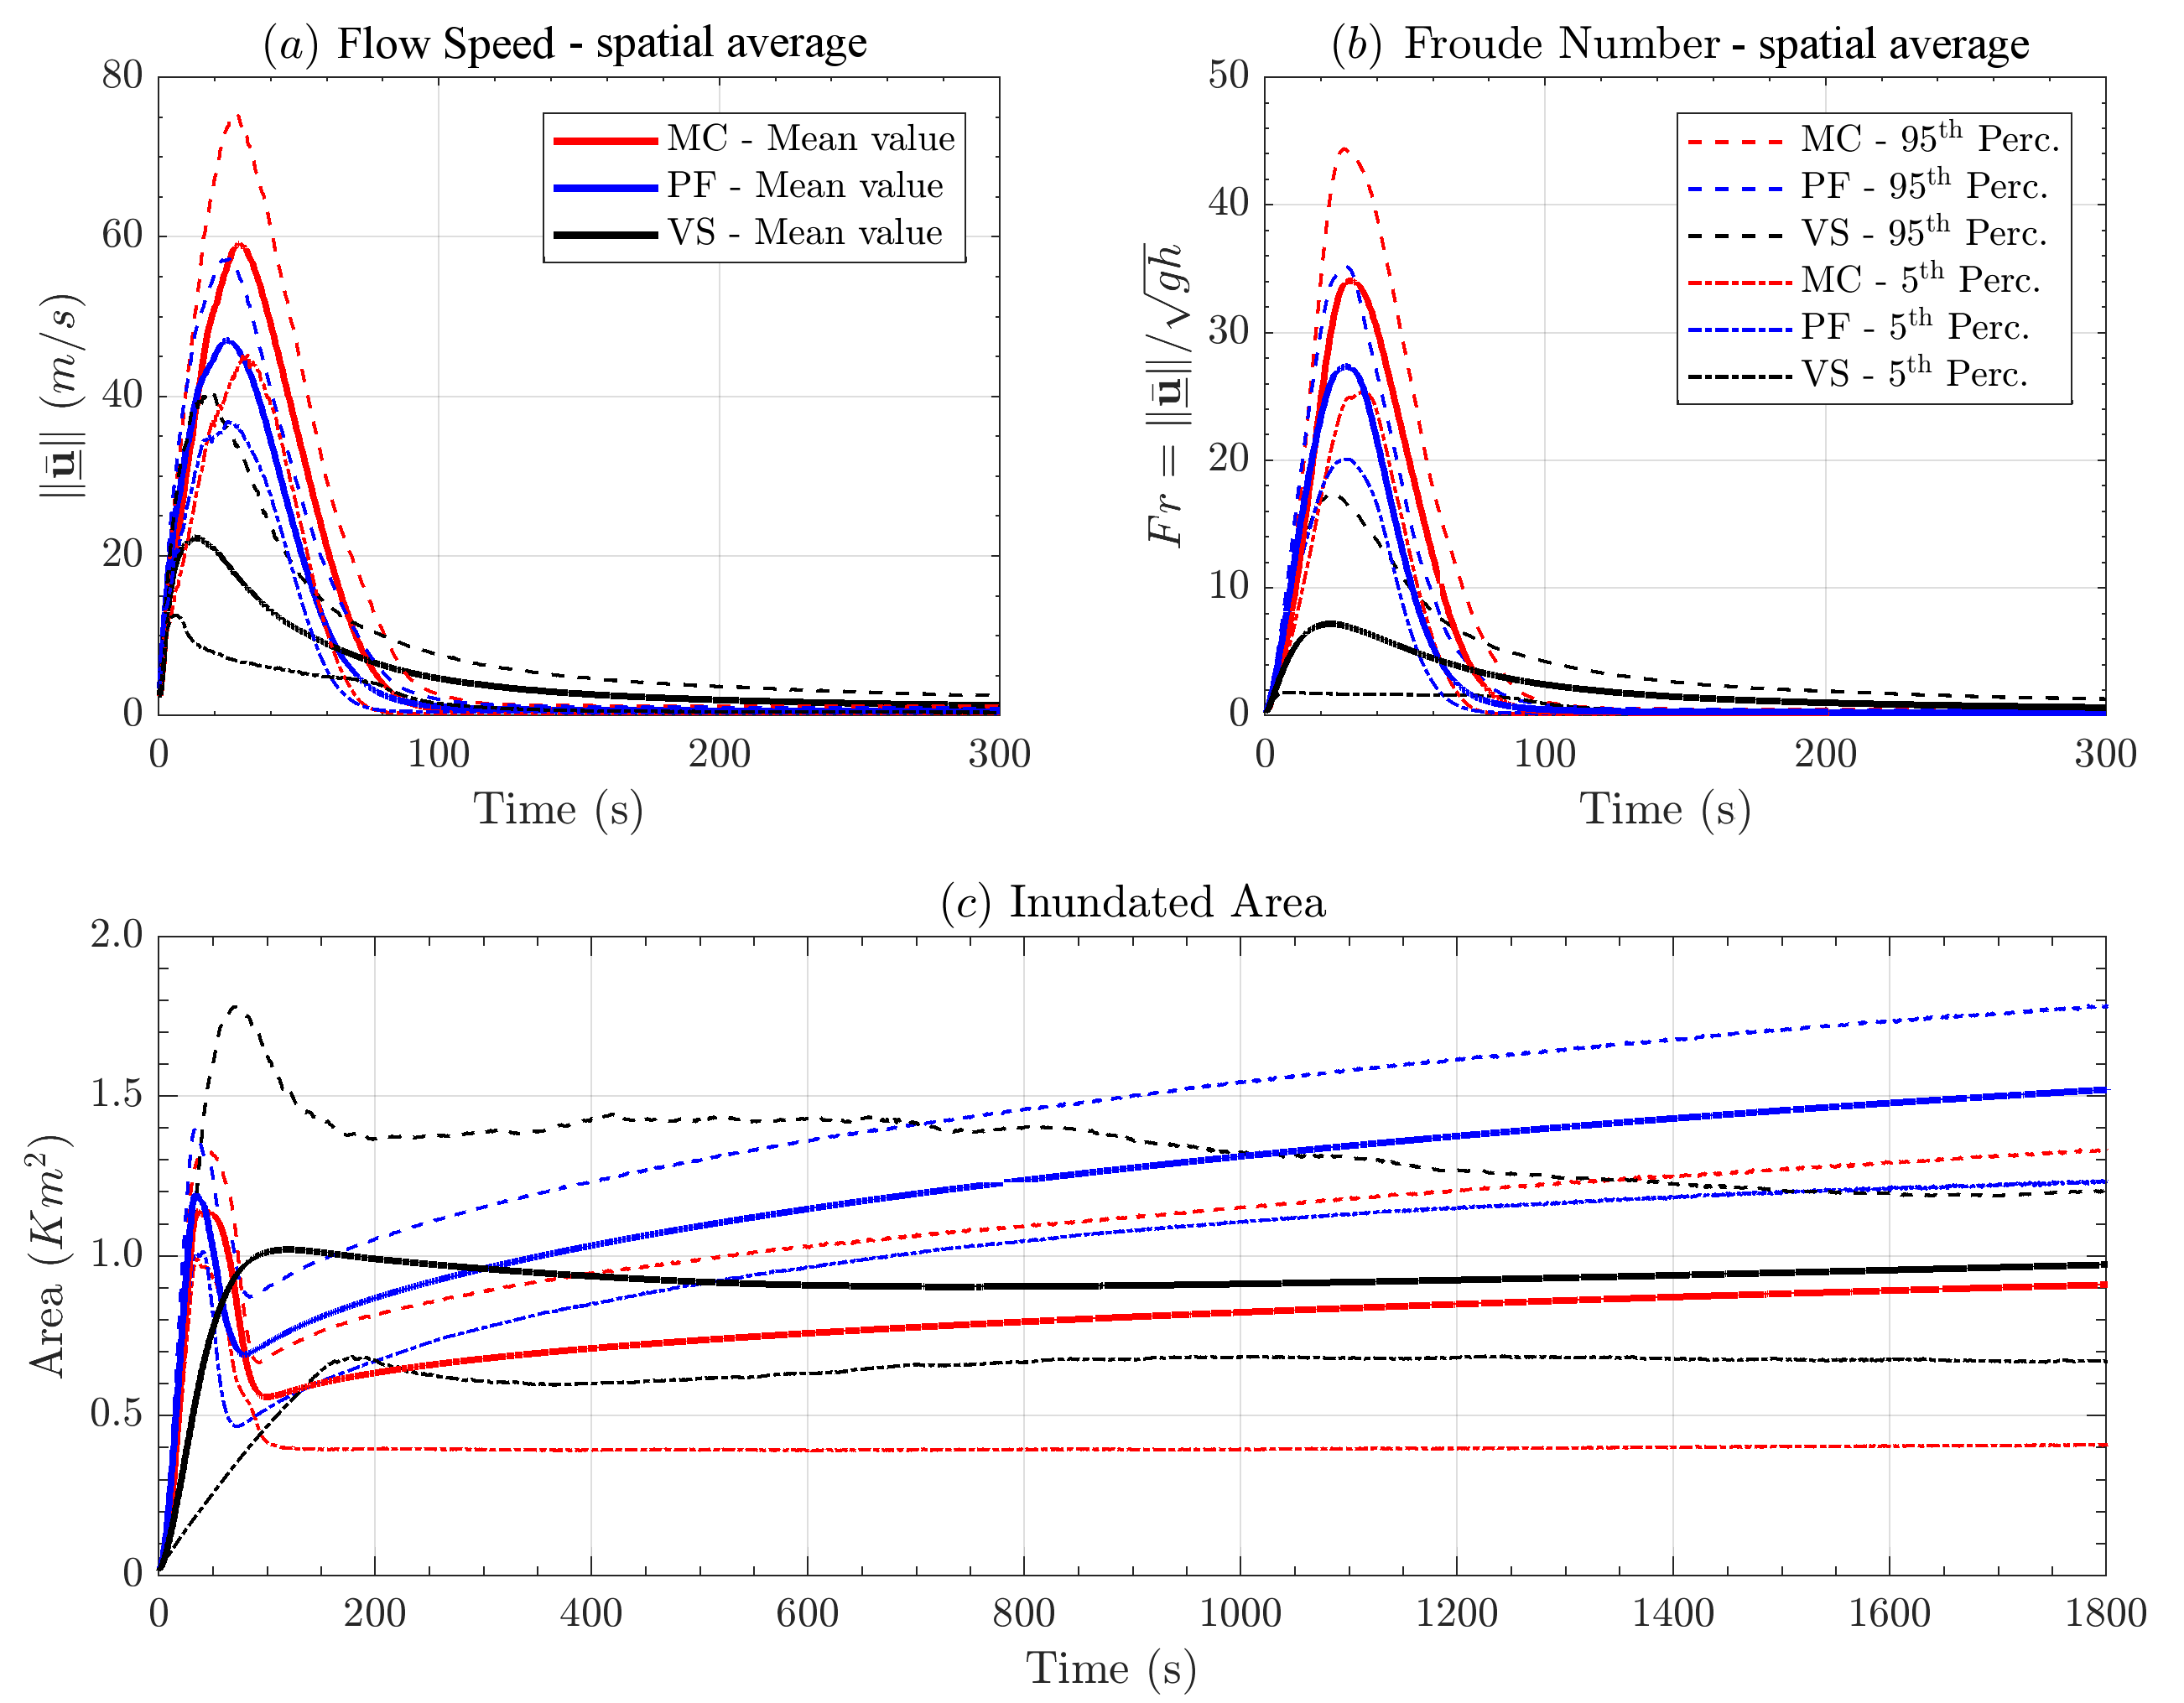
\includegraphics[width=0.75\textwidth]{figures/Colima/AveragedColima.png}
        \caption{Comparison between spatial averages of $(a)$ flow speed, and $(b)$ Froude Number, in addition to the $(c)$ inundated area, as a function of time. Bold line is mean value, dashed/dotted lines are 5$^{\mathrm{th}}$ and 95$^{\mathrm{th}}$ percentile bounds. Different models are displayed with different colors.}
\end{figure}
\end{frame}


\begin{frame}
\frametitle{Conclusions}
\begin{itemize}
  \item our approach evaluates the statistics of a range of simulations, produced by the couple $\left(M, P_M\right)$.
\vskip.3cm
  \item the new statistical framework processes the mean and the uncertainty range of either observable or latent variables in the simulation. 
\vskip.3cm
  \item analysis is performed at selected sites, and spatial integrals were also performed, illustrating the characteristics of the entire output.
\vskip.3cm
  \item the new concepts of dominance factors and expected contributions, enable a simplified description of the local dynamics. 
\end{itemize}
\end{frame}

\end{document}
